\documentclass[a4paper, 11pt, oneside]{article}

\usepackage[utf8]{inputenc}
\usepackage[T1]{fontenc}
\usepackage[english]{babel}
\usepackage{array}
\usepackage{shortvrb}
\usepackage{listings}
\usepackage[fleqn]{amsmath}
\usepackage{amsfonts}
\usepackage{fullpage}
\usepackage{enumerate}
\usepackage{enumitem}
\usepackage{graphicx}
\usepackage{subfigure}
\usepackage{alltt}
\usepackage{indentfirst}
\usepackage{eurosym}
\usepackage{listings}
\usepackage{titlesec, blindtext, color}
\usepackage{float}
\usepackage[colorlinks, linkcolor=blue]{hyperref}
\usepackage[nameinlink,noabbrev]{cleveref}

\usepackage{titling}
\renewcommand\maketitlehooka{\null\mbox{}\vfill}
\renewcommand\maketitlehookd{\vfill\null}

\definecolor{mygray}{rgb}{0.5,0.5,0.5}
\definecolor{pink1}{rgb}{0.858, 0.188, 0.478}
\definecolor{sienna}{rgb}{0.53, 0.18, 0.09}
\definecolor{sepia}{rgb}{0.44, 0.26, 0.08}
\definecolor{midnightblue}{rgb}{0.1, 0.1, 0.44}

\newcommand{\ClassName}{INFO-0027: Programming Techniques}
\newcommand{\ProjectName}{Project 2: File Explorer - Report}
\newcommand{\AcademicYear}{2020 - 2021}

%%%% Page de garde %%%%

\title{\ClassName\\\vspace*{0.8cm}\ProjectName\vspace{0.8cm}}
\author{Goffart Maxime \\180521 \and Joris Olivier \\ 182113}
\date{\vspace{1cm}Academic year \AcademicYear}

\begin{document}

\begin{titlingpage}
{\let\newpage\relax\maketitle}
\end{titlingpage}

%%%%%%%%%%%%%%%%%%%%%%%%%%%%%%%%%%%%%%%%%%%%%%

\section{Software architecture}

\subsection{Creational patterns}

\paragraph{}We chose to use the factory method pattern to create the classes representing the different entities that the file manager manipulates (files, folders, aliases, and archives).
We chose to use this pattern because all the entities are sharing the same properties (name, children, parent, etc). In this way,  we can easily add new types of entities to the project and the task of choosing which entity to build is performed dynamically by the creators.

The advantages of using this pattern are that we can easily modify our code because the object creation is modular, we do not have code repetitions while instantiating an object, and new types of concrete products can easily be added to the code.

The drawback is that the class hierarchy is a bit complex for its usage in our case.

\paragraph{}We also use the singleton pattern for the concrete creator classes in order to be sure that they cannot be instantiated more than once and avoiding global variables.

The advantage of this pattern is that it ensures that there is only a single concrete creator for each corresponding entity.

The drawback of this pattern is that it can lead to break the single responsibility principle.

\paragraph{}The UML static diagram representing these patterns can be observed on the \autoref{fig:creational}

\begin{figure}[!ht]
    \centering
    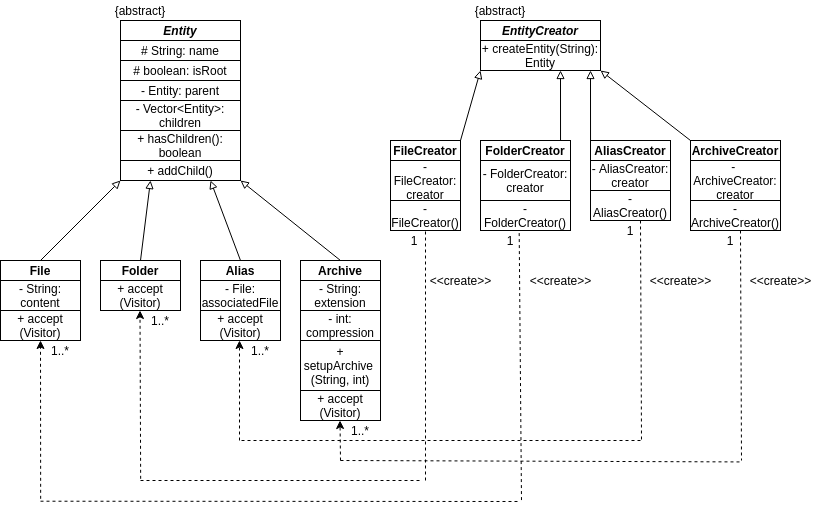
\includegraphics[scale=0.6]{creationnal.png}
    \caption{UML static diagram of the classes related to creational patterns.}\label{fig:creational}
\end{figure}

\subsection{Structural patterns}

\paragraph{}We chose to use the adapter pattern because we do not have access to the source code related to the \texttt{TextAreaManager} and \texttt{ExplorerSwingView} classes but we wanted to add some functionalities related to these classes. For instance, we wanted to manipulate the tree that represents the view of the file manager and texts.

The advantages of using this pattern is that it allows to reuse and adapt to our needs the interface implemented in the \texttt{graphics.jar} file without having access to it and modifying it.

The drawback is that the code complexity is increased. In fact, we can need many adaptation levels to reach the desired type. 

\paragraph{}The UML static diagram representing this pattern can be observed on the \autoref{fig:structural}

\begin{figure}[H]
    \centering
    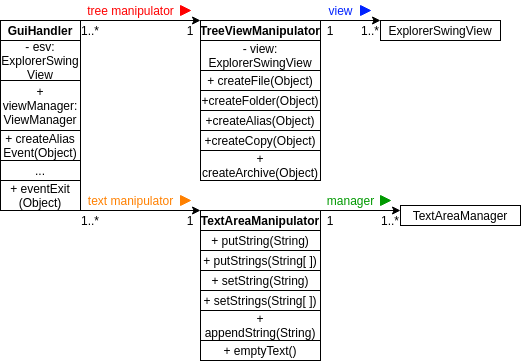
\includegraphics[scale=0.6]{structural.png}
    \caption{UML static diagram of the classes related to structural patterns.}\label{fig:structural}
\end{figure}

\subsection{Behavioral patterns}

\paragraph{}We decided to use the visitor pattern for the copy, the display, and the building of an archive because, with this pattern, these new operations can easily be added and without modifying the code related to these entities.

The advantage is that this pattern allows to easily add such new operations.

The drawback is that the structure of composite objects is complex to modify and can lead to encapsulation problems.

\paragraph{}The UML static diagram representing this pattern can be observed on the \autoref{fig:behavioral}

\begin{figure}[H]
    \centering
    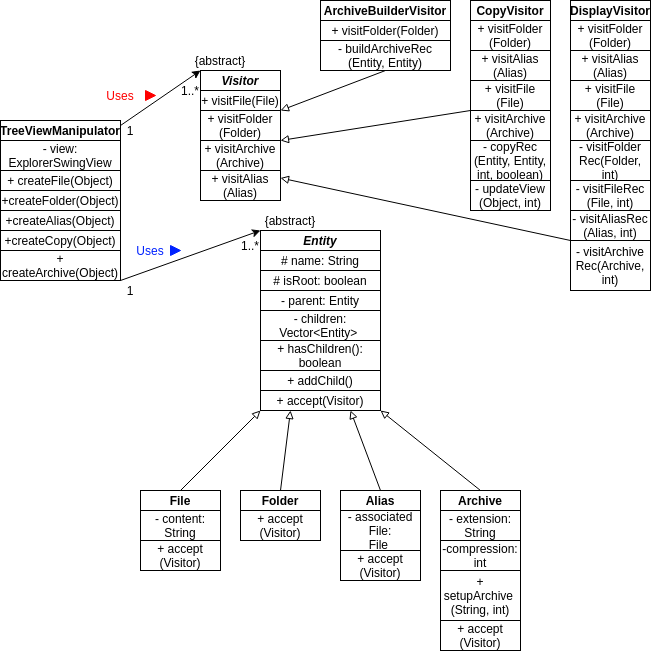
\includegraphics[scale=0.6]{behavioral.png}
    \caption{UML static diagram of the classes related to behavioral patterns.}\label{fig:behavioral}
\end{figure}

\section{Feedback}

Olivier spent about 12 hours on the project while Maxime, on his side, spent about 12 hours on it.


\end{document}
